\scanpage{19}

passage du carré aux deux tétraèdres

\figure{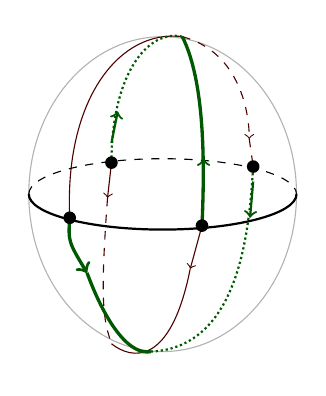
\begin{tikzpicture}[scale=1]
\draw[gray!60] (0,0) ellipse (1.7 and 2);
\draw[thick] (-1.7,0) arc[start angle=180,end angle=360,x radius=1.7,y radius=.45];
\draw[dashed] (-1.7,0) arc[start angle=180,end angle=0,x radius=1.7,y radius=.45];
\draw[red!30!black] (-1.18,-.3)..controls(-1.25,1.2)and(-.55,2.1)..(.25,2);
\draw[red!30!black,dashed,->] (.25,2)..controls(1,1.8)and(1.1,1)..(1.1,.7);
\draw[red!30!black,dashed] (1.1,.7)--(1.15,.35);
\draw[red!30!black,->] (.5,-.4)--(.35,-.95);
\draw[red!30!black] (.35,-.95)..controls(.1,-2.2)and(-.4,-2.1)..(-.65,-1.9);
\draw[red!30!black,->] (-.65,.4)--(-.7,-.05);
\draw[red!30!black,dashed] (-.7,-.05)..controls(-.8,-1.4)and(-.75,-1.6)..(-.65,-1.9);
\draw[green!35!black,very thick] (.25,2)..controls(.55,1.4)and(.53,.3)..(.5,-.4);
\draw[green!35!black,->,thick] (.52,.05)--(.52,.45);
\draw[green!35!black,densely dotted,thick] (-.65,.4)..controls(-.65,1.5)and(-.2,2.1)..(.25,2);
\draw[green!35!black,->,thick] (-.65,.65)--(-.57,1.05);
\draw[green!35!black,very thick,->] (-1.18,-.3)..controls(-1.2,-.6)..(-.96,-1);
\draw[green!35!black,very thick] (-.96,-1)..controls(-.7,-1.7)and(-.4,-2.05)..(-.15,-2);
\draw[green!35!black,densely dotted,thick] (-.15,-2)..controls(1,-1.95)and(1.1,-.4)..(1.15,.35);
\draw[green!35!black,->,thick] (1.15,.16)--(1.11,-.3);
\foreach \p in {(-1.18,-.3),(.5,-.4),(-.65,.4),(1.15,.35)}{\fill \p circle (.08);}
\end{tikzpicture}}

Pour avoir le passage \unsure{aux autres} structures pantaloniques, il faut introduire la \deleted{\unsure{double}}\unsure{subdivision} barycentrique complète de la carte carrée.

dans les deux cas \inserted{``\unsure{spéciaux}''} non dégénérés (carré, tétraèdre) les frontières adjacentes sont \deleted{\unsure{toutes}} ``contenues dans la subdivision barycentrique

\begin{flushright}
\texttt{NS 001 072}\\
\texttt{L ===> PAGE}\\
\texttt{************}
\end{flushright}

\figure{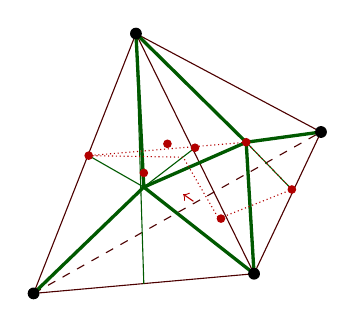
\begin{tikzpicture}[scale=1]
\coordinate (A) at (0,0); \coordinate (B) at (1.3,3.3);
\coordinate (C) at (2.8,.25); \coordinate (D) at (3.65,2.05);
\coordinate (O) at (1.4,1.35); \coordinate (P) at (2.7,1.92);
\draw[red!30!black] (A)--(B)--(C)--(D)--(B);
\draw[red!30!black] (A)--(C);
\draw[red!30!black,dashed] (A)--(D);
\draw[green!35!black,very thick] (B)--(O)--(A) (O)--(C) (O)--(P)--(D) (B)--(P)--(C);
\draw[green!35!black] (B)--(1.4,.12) (.7,1.75)--(O)--(2.05,1.85) (2.7,1.92)--(3.28,1.32);
\draw[red!70!black,densely dotted] (.7,1.75)--(1.9,1.73)--(2.35,.95)--(3.28,1.32)--(2.7,1.92)--cycle;
\foreach \p in {A,B,C,D}{\fill (\p) circle (.075);}
\foreach \p in {(.7,1.75),(1.4,1.53),(2.05,1.85),(2.7,1.92),(3.28,1.32),(1.7,1.9),(2.38,.95)}{\fill[red!70!black] \p circle (.055);}
\draw[red!70!black,->] (2.03,1.17)--(1.9,1.26);
\end{tikzpicture}}

cette carte \inserted{\unsure{commune}} (subdivision bar. du tétraèdre) contient également les subdivisions barycentriques des trois \unsure{coins|cas} ``carrés'' associés, (dont l'une est marquée en pointillés rouges)

\figure{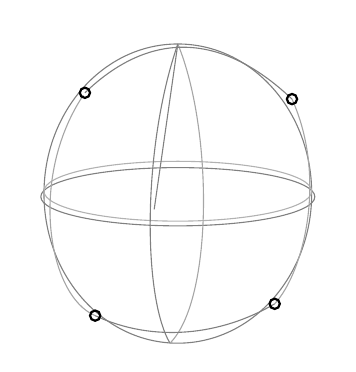
\begin{tikzpicture}[scale=1]
\draw[gray] (0,0) ellipse (1.7 and 1.9);
\draw[gray] (0,-.04) ellipse (1.74 and .37);
\draw[gray!60] (0,.03) ellipse (1.7 and .38);
\draw[gray] (0,1.9)..controls(-.45,.6)and(-.45,-1.3)..(-.1,-1.9);
\draw[gray!70] (0,1.9)..controls(.45,.8)and(.45,-1.35)..(-.1,-1.9);
\draw[gray] (-1.18,1.28)..controls(-.4,2.03)and(.5,2.1)..(1.45,1.2);
\draw[gray] (-1.05,-1.55)..controls(-.3,-1.9)and(.55,-1.8)..(1.23,-1.4);
\draw[gray!70] (-1.2,1.25)..controls(-1.9,.2)and(-1.65,-1.3)..(-1.05,-1.55);
\draw[gray!70] (1.45,1.2)..controls(1.9,.2)and(1.6,-1)..(1.23,-1.4);
\foreach \p in {(-1.18,1.28),(1.45,1.2),(-1.05,-1.55),(1.23,-1.4)}{\draw[thick] \p circle (.065);}
\draw[gray] (0,1.9)--(-.3,-.2);
\end{tikzpicture}}

\margin{18}
